%\begin{figure}
%\centering
%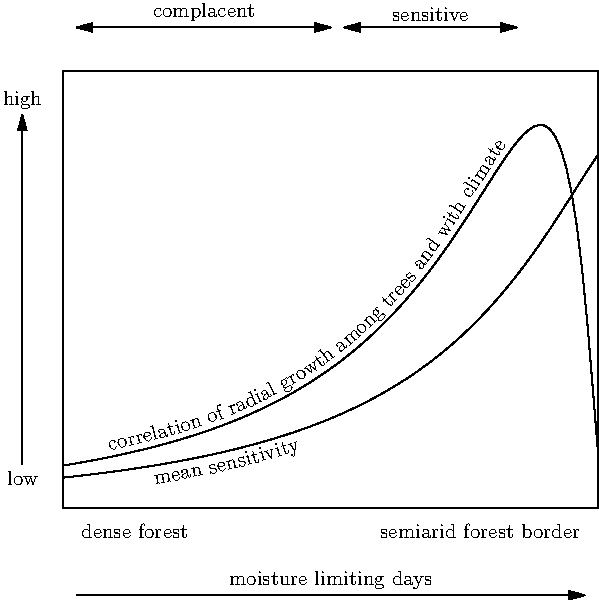
\includegraphics[width=6in]{figures/fritts.pdf}
%\caption{A simplified rendition of the diagram originally seen in \cite{fritts1976tree}.}
%\label{fig:fritts}
%\end{figure}

\begin{figure}
\centering
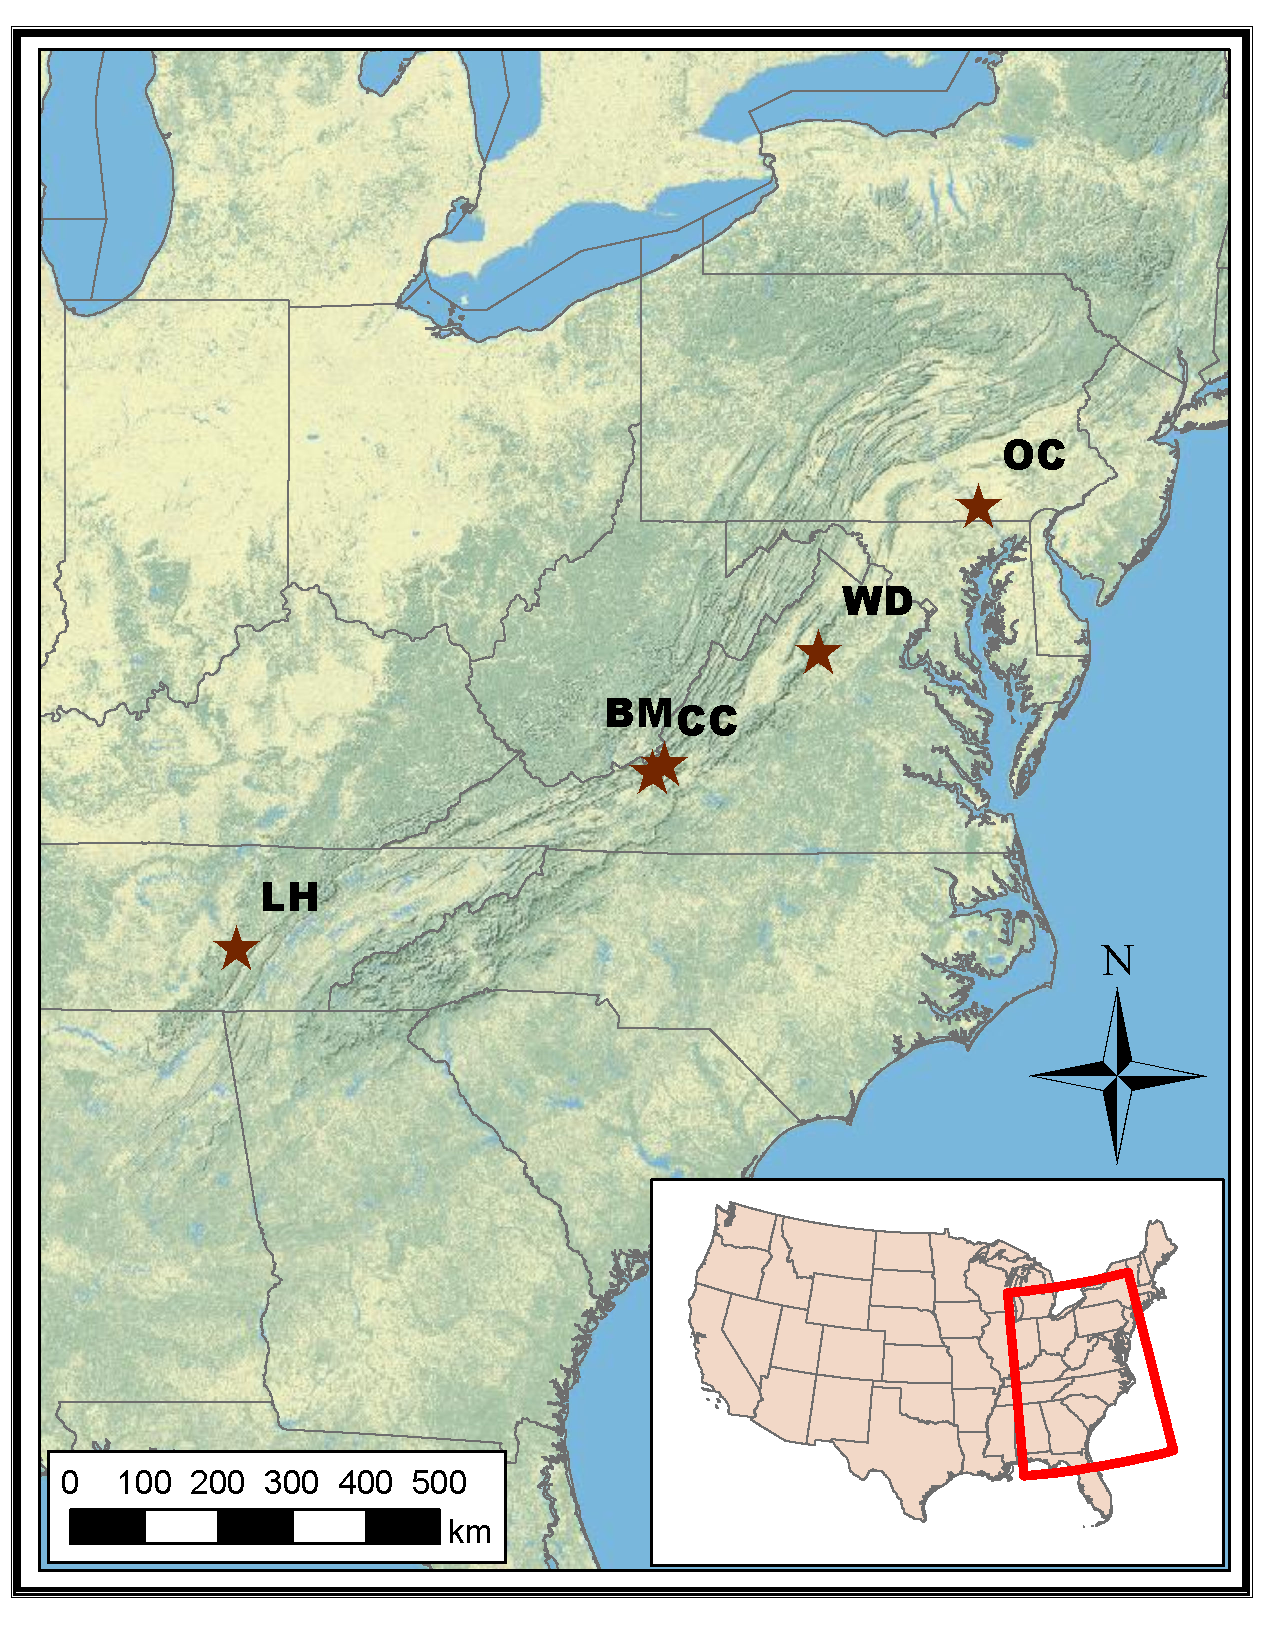
\includegraphics[width=6in]{figures/NewClimateNADEF.pdf}
\caption{Regional chronology sample locations.}
\label{fig:map}
\end{figure}

\begin{figure}
\centering
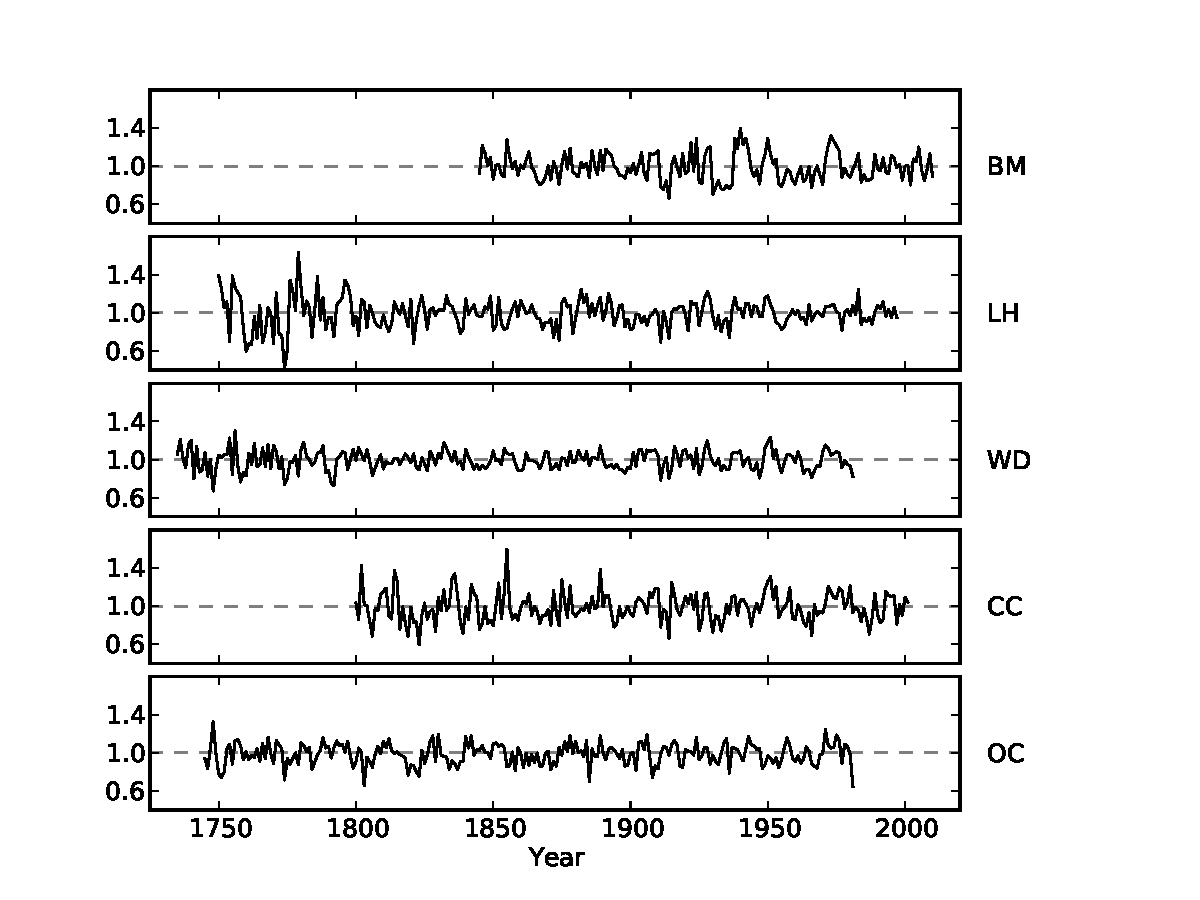
\includegraphics[width=6in]{figures/stacked_chrons.pdf}
\caption{Plots of the five chronologies used in the principal component analysis. The top panel shows the chronology built from the sample data at Brush Mountain (BM), while the others are the regional chronologies from Lynn Hollow (LH), watchdog Mountain (WD), Craig Creek (CC), and Otter Creek (OC).}
\label{fig:stackedChrons}
\end{figure}

\begin{figure}
\centering
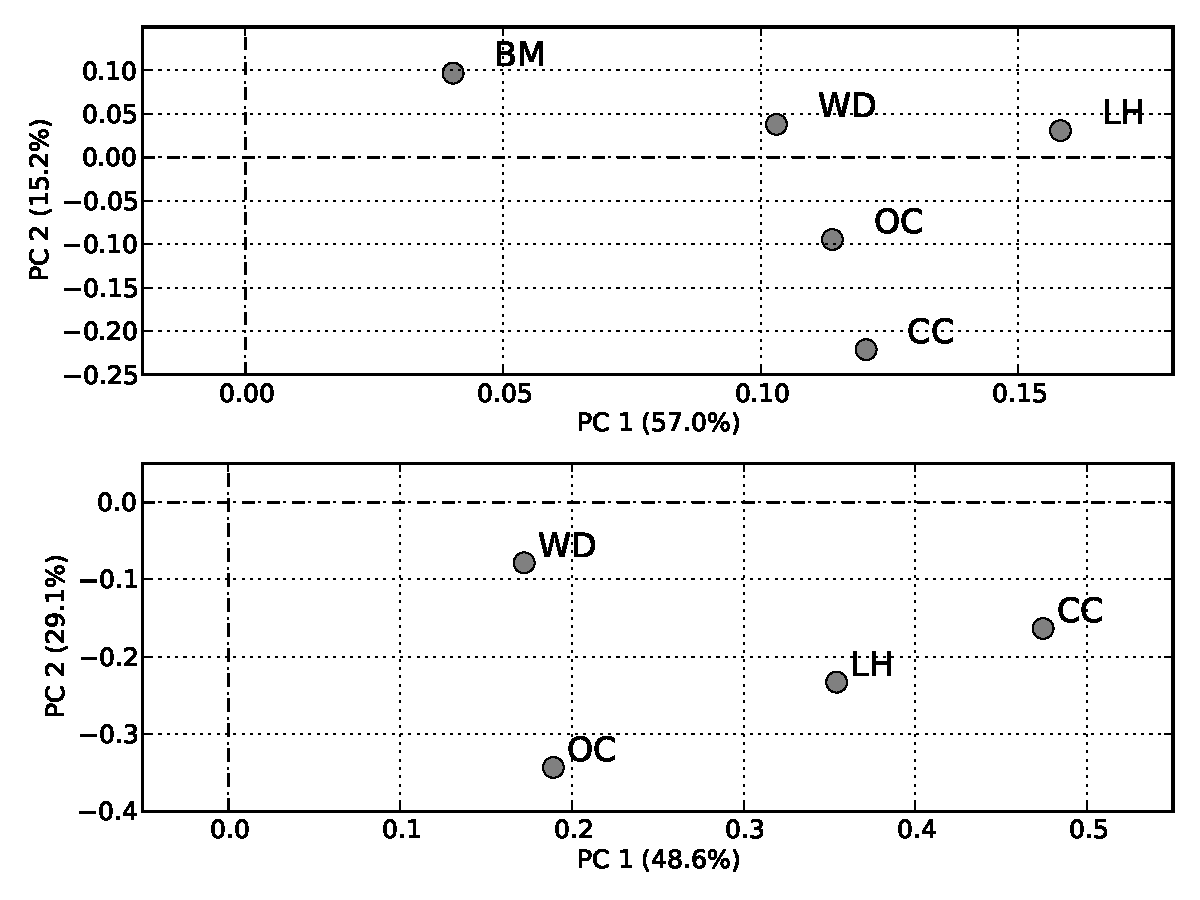
\includegraphics[width=6in]{figures/scoresPlot.pdf}
\caption{Plot showing the sample site scores when plotted on the First principal component versus second principal component axes.}
\label{fig:scores}
\end{figure}

\begin{figure}
\centering
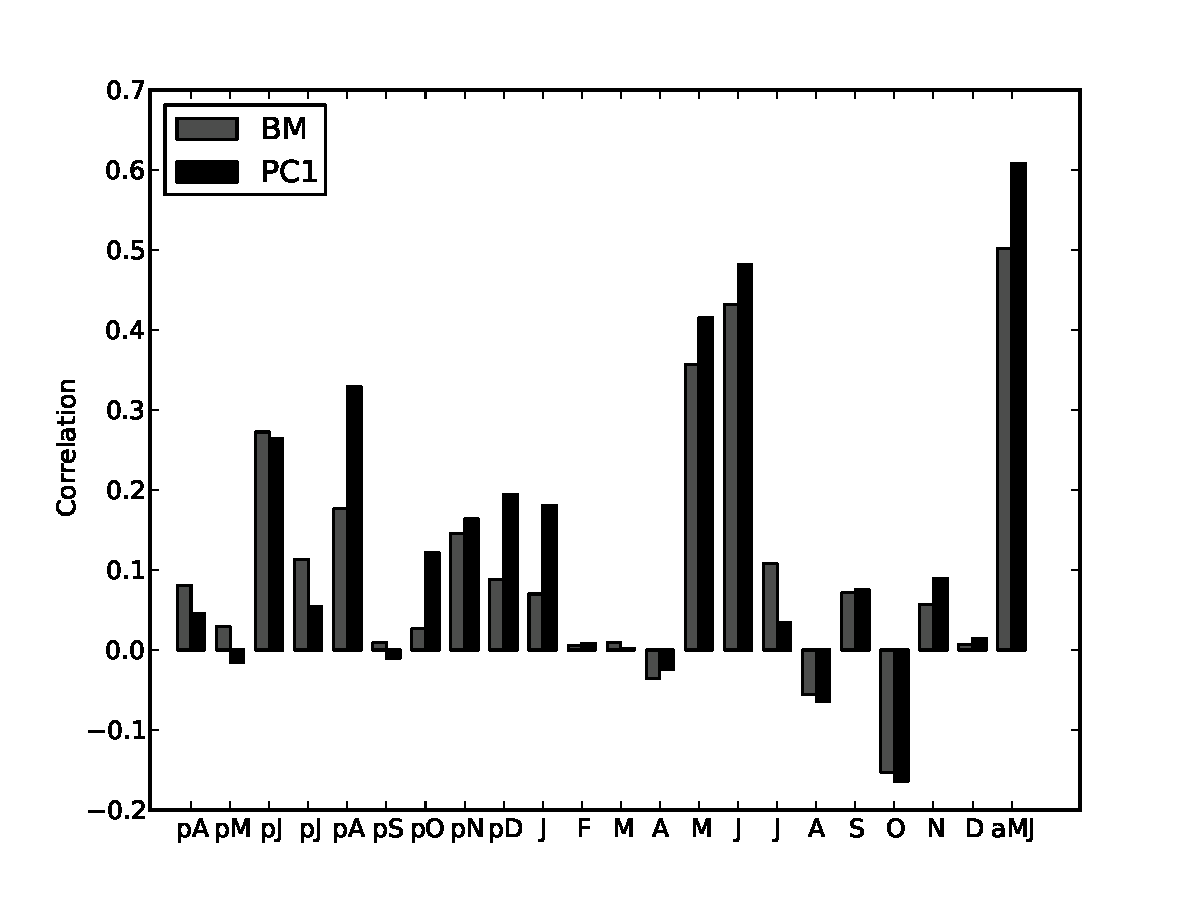
\includegraphics[width=6in]{figures/climCorrPrecip.pdf}
\caption{Correlation between the growth proxies (BM or PC1) and the monthly precipitation from previous April (pA) through December (D) as well as for averaged May and June (aMJ).}
\label{fig:precipBarCorr}
\end{figure}

\begin{figure}
\centering
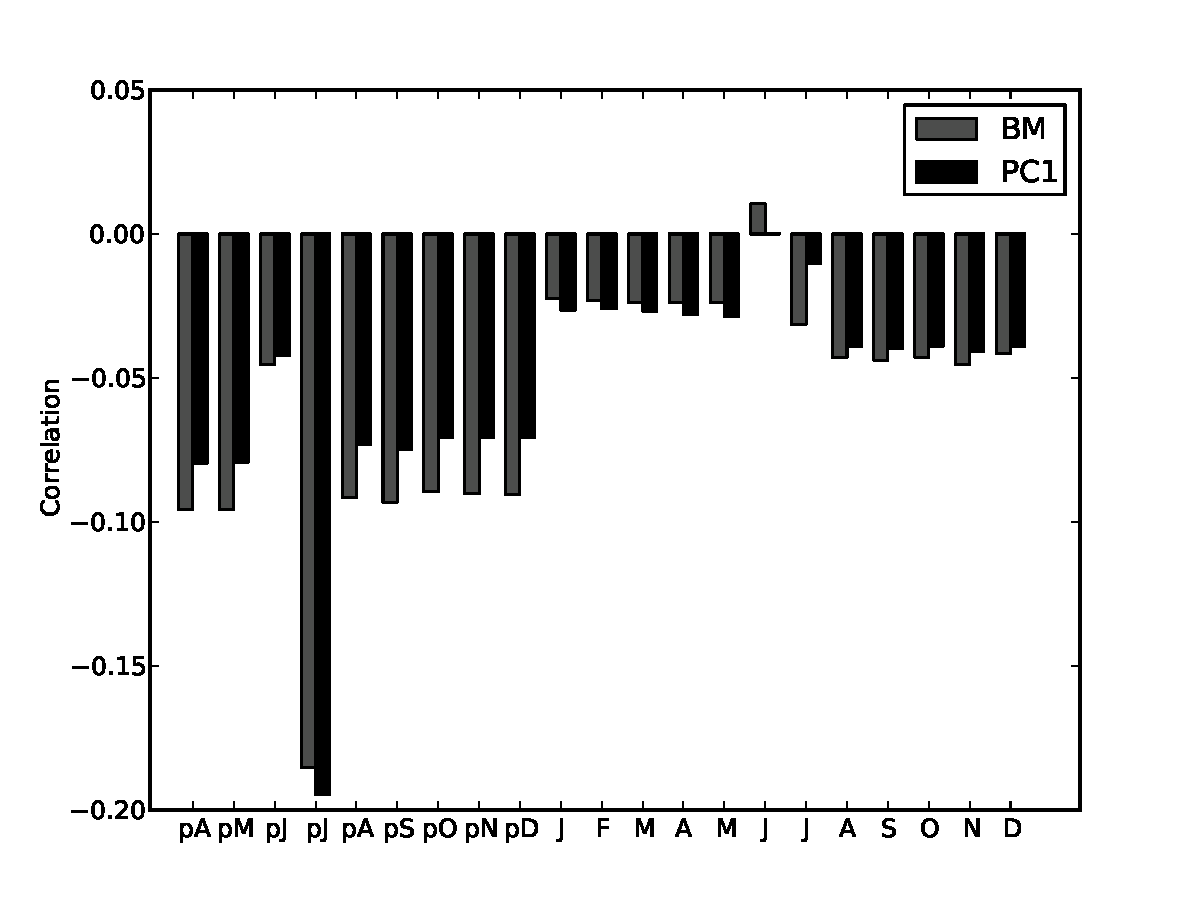
\includegraphics[width=6in]{figures/climCorrTemp.pdf}
\caption{Correlation between the growth proxies (BM or PC1) and average monthly temperature from previous April (pA) through December (D).}
\label{fig:tempBarCorr}
\end{figure}

\begin{figure}
\centering
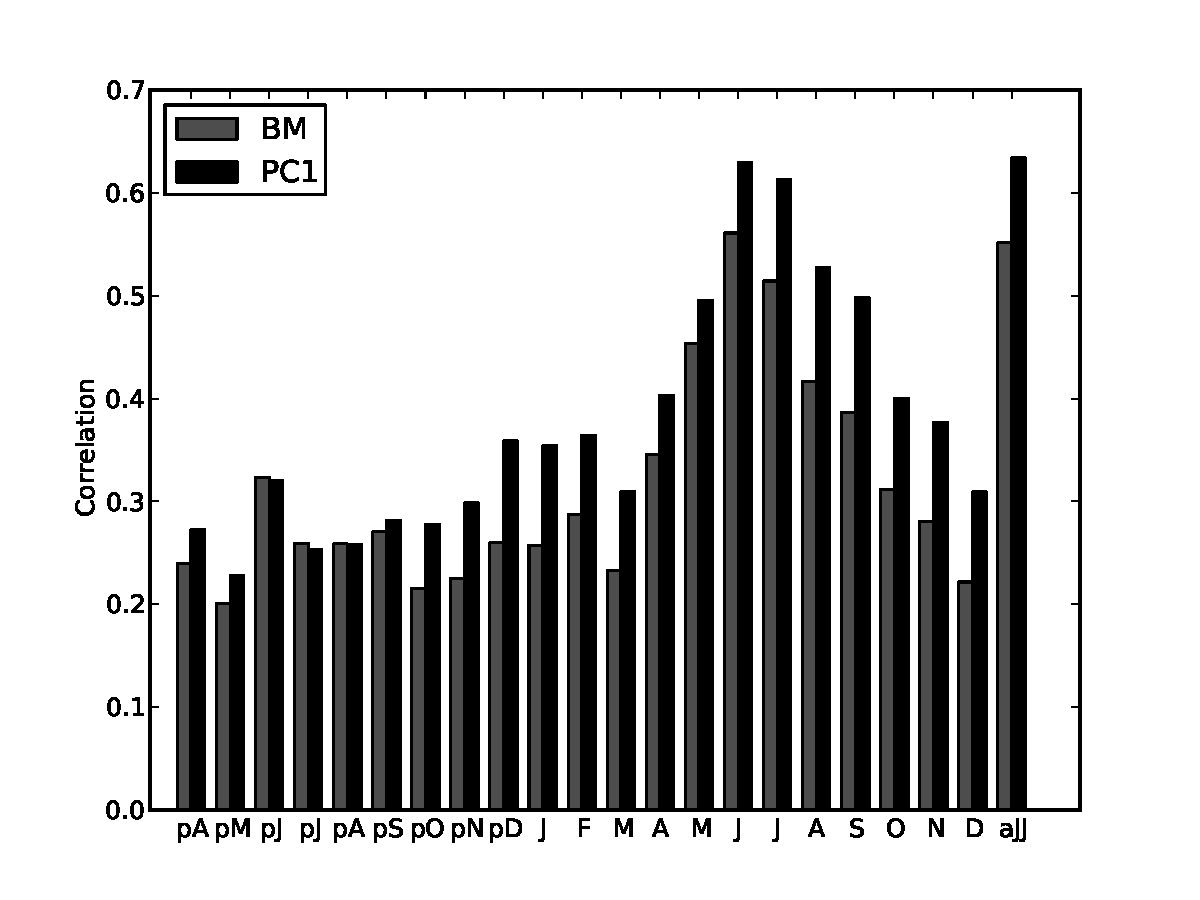
\includegraphics[width=6in]{figures/climCorrPdsi.pdf}
\caption{Correlation between the growth proxies (BM or PC1) and average PDSI from previous April (pA) through December (D) as well as for averaged June and July (aJJ).}
\label{fig:pdsiBarCorr}
\end{figure}

\begin{figure}
\centering
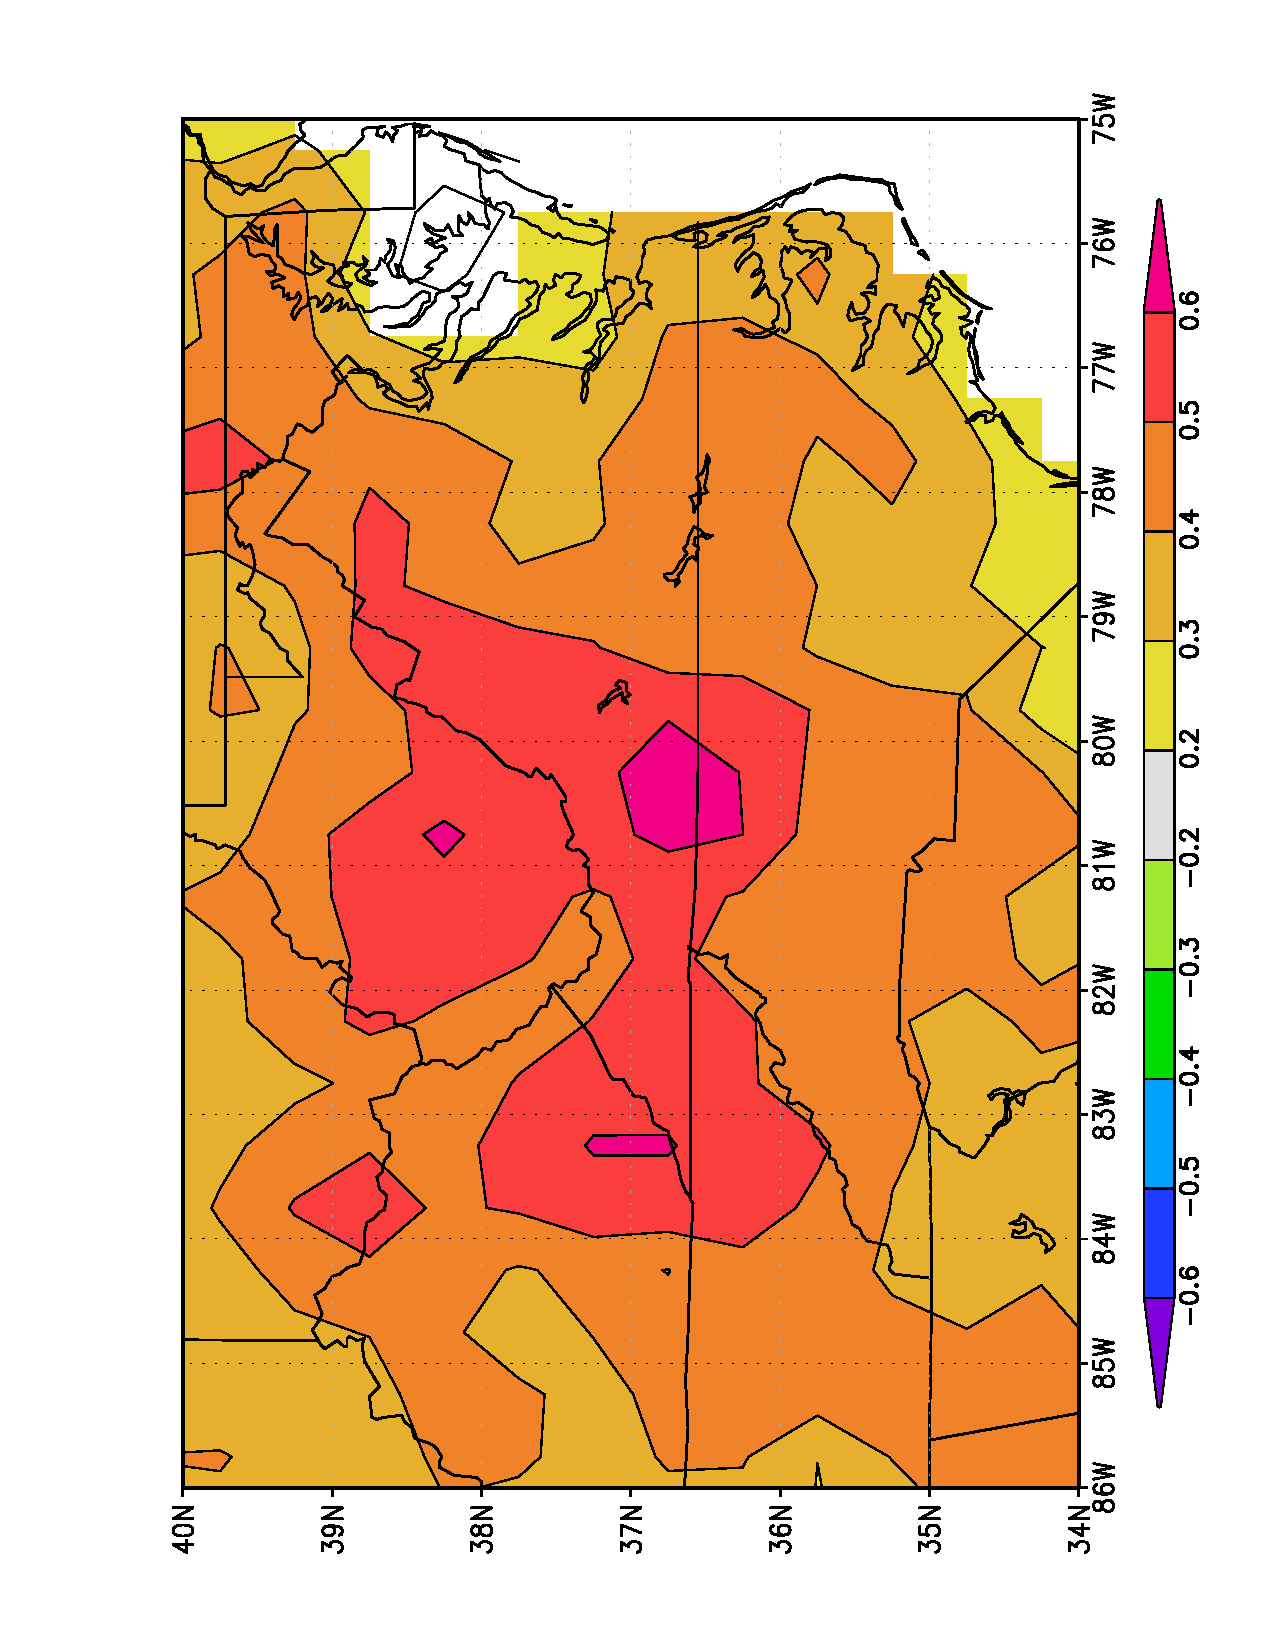
\includegraphics[width=5in, angle=-90]{figures/corrMapPrecipMJ.pdf}
\caption{Correlation map showing the correlation between the first principal component and averaged June July PDSI (jjPDSI).}
\label{fig:precipCorrMap}
\end{figure}

\begin{figure}
\centering
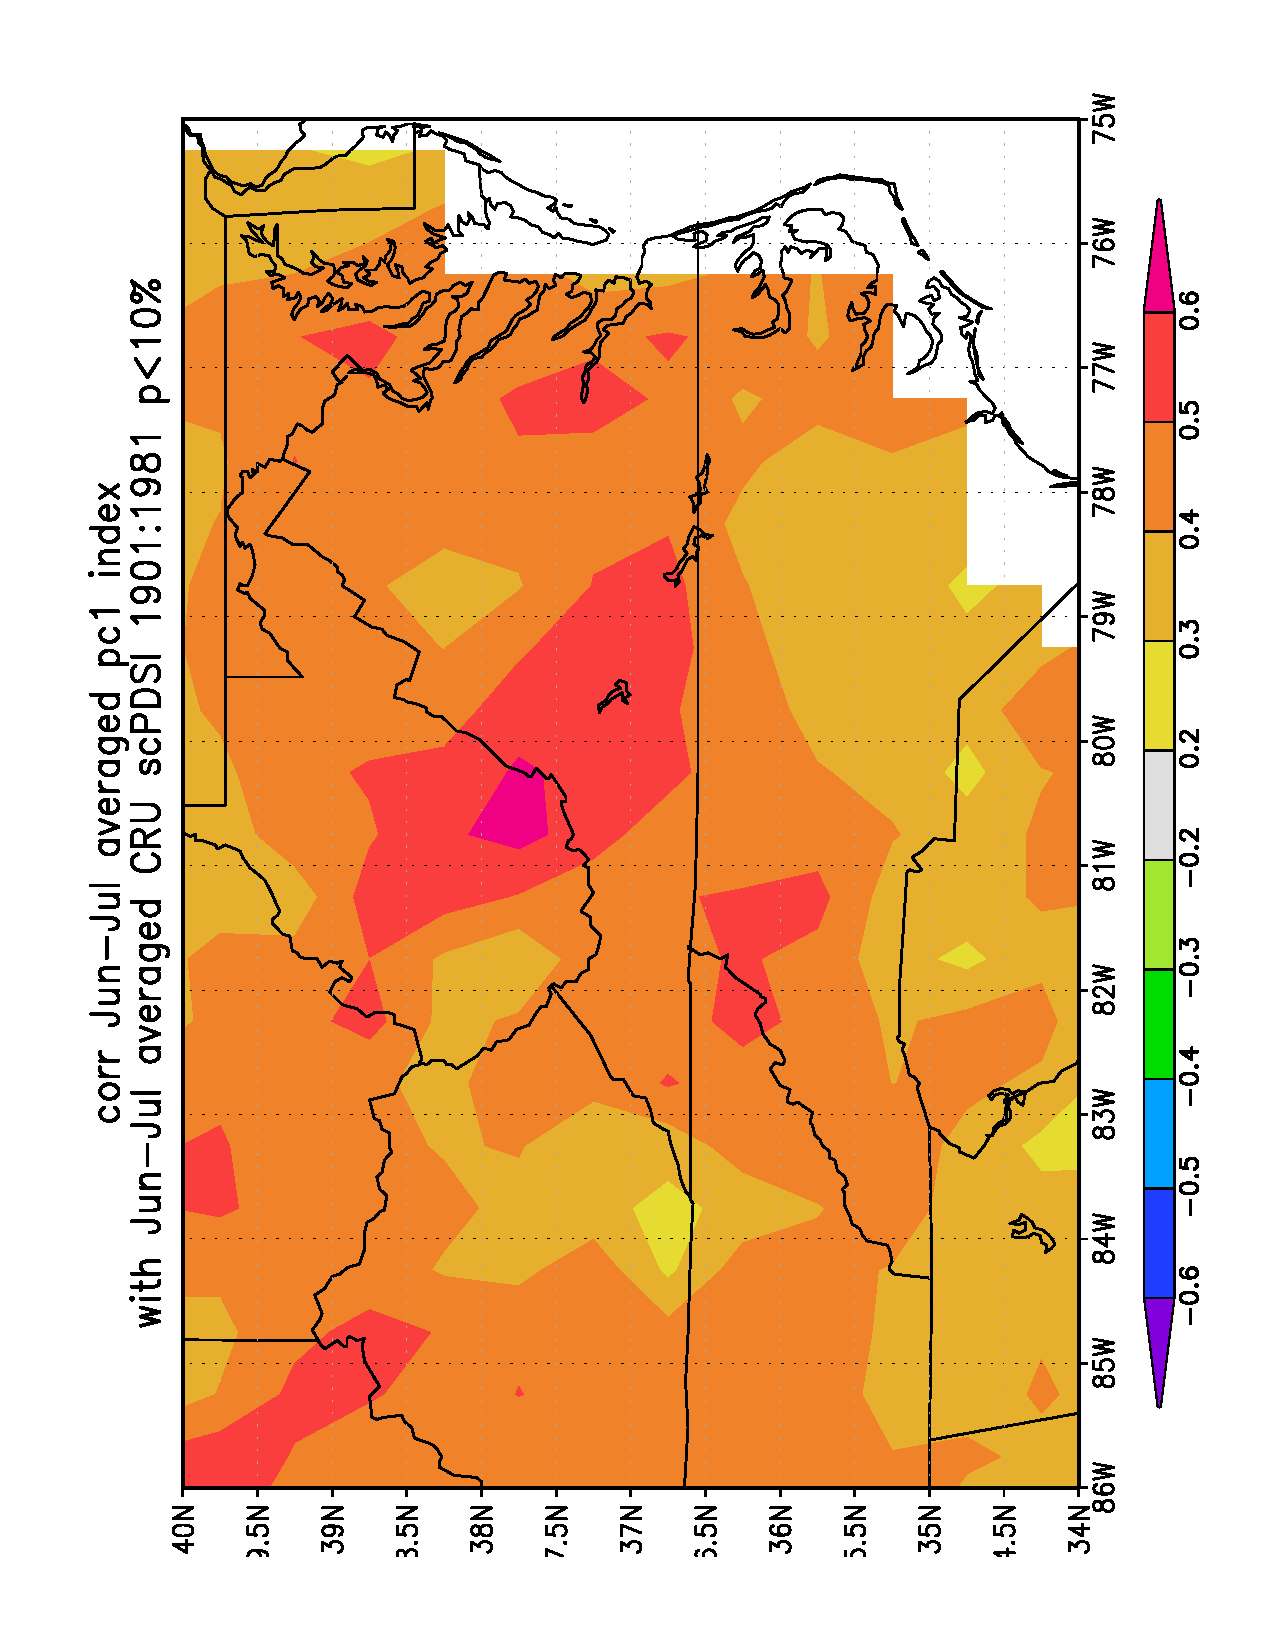
\includegraphics[width=5in, angle=-90]{figures/corrMapPdsiJJ.pdf}
\caption{Correlation map.}
\label{fig:pdsiCorrMap}
\end{figure}

\begin{figure}
\centering
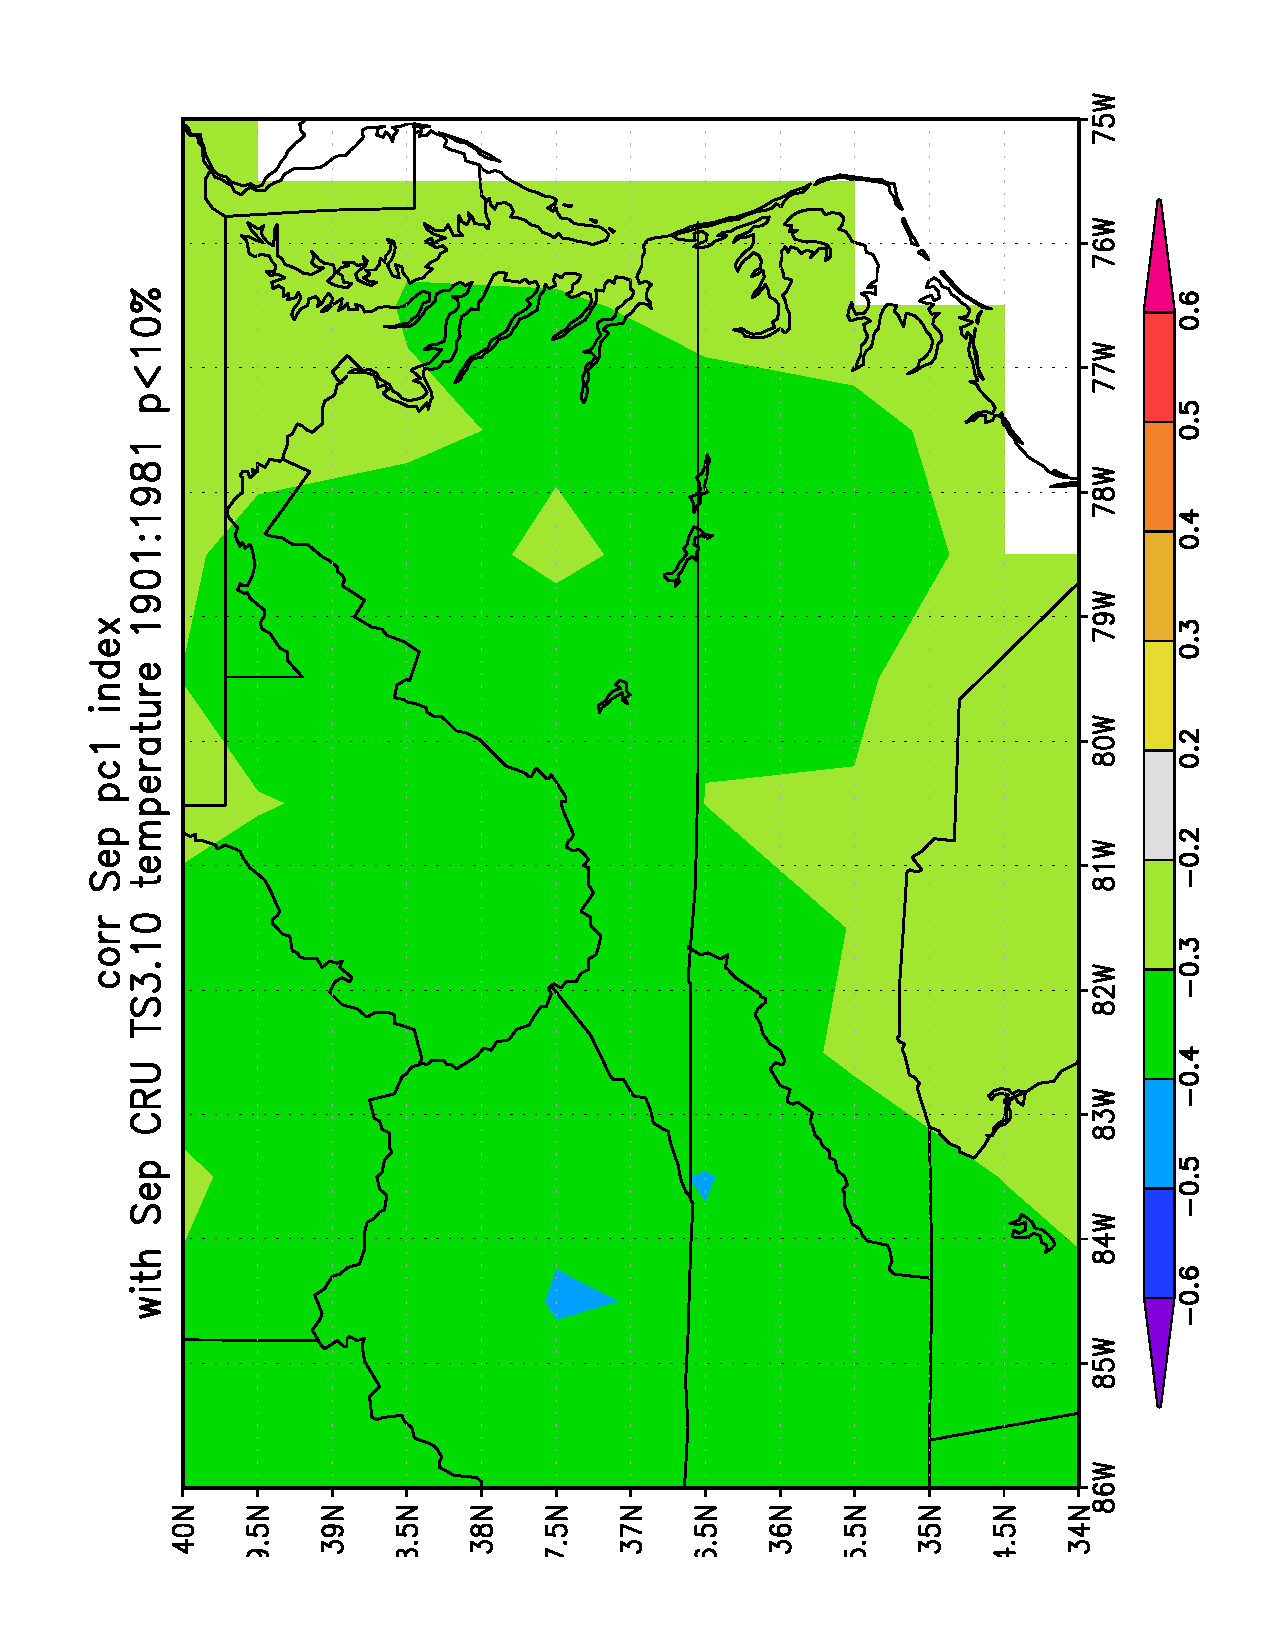
\includegraphics[width=5in, angle=-90]{figures/corrMapTempSept.pdf}
\caption{Correlation map showing the correlation between the first principal component and September temperature.}
\label{fig:tempCorrMap}
\end{figure}

\begin{figure}
\centering
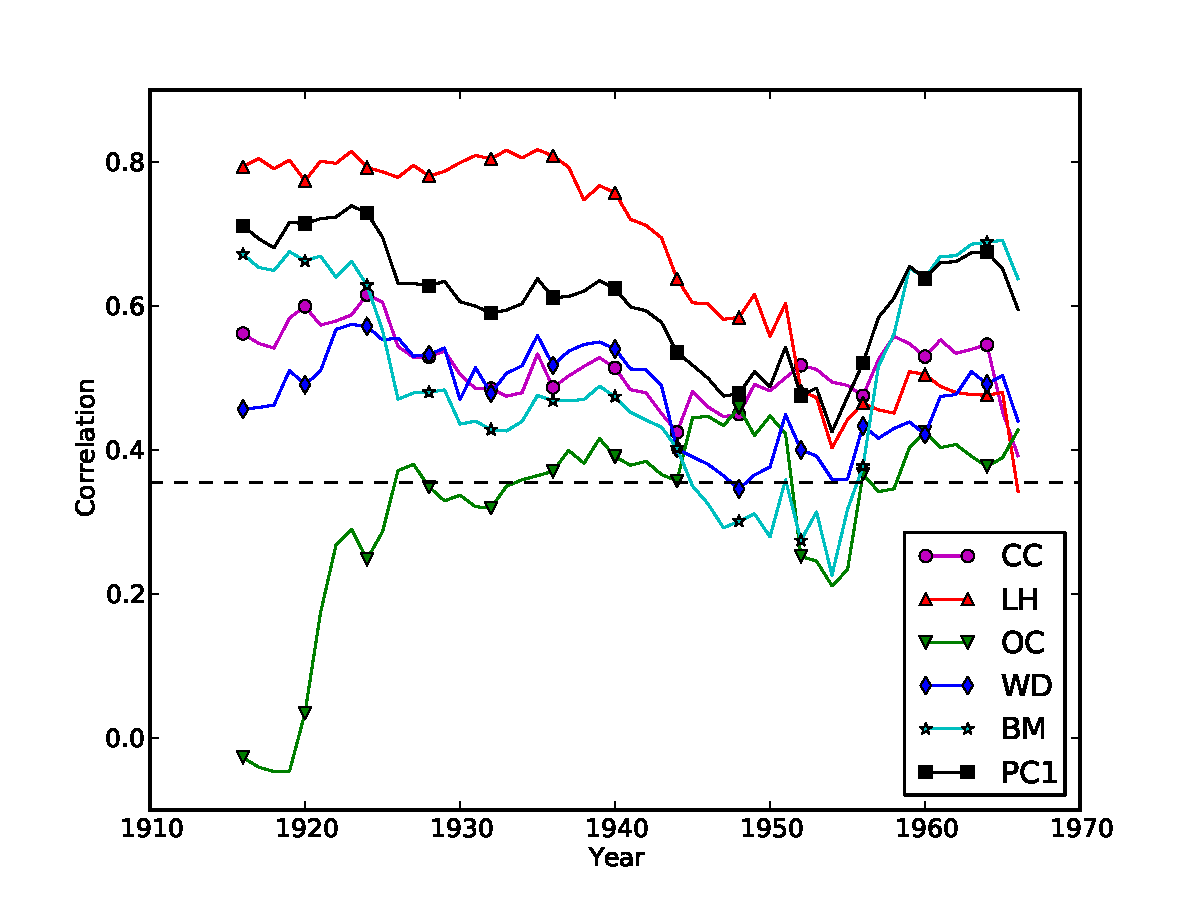
\includegraphics[width=5in]{figures/precipRunningCorr.pdf}
\caption{A 31-year windowed correlation plot showing the correlations between each growth proxy (chronologies and first principal component) and mjPR. Correlation points are plotted above the window centers.}
\label{fig:precipRunningCorr}
\end{figure}

\begin{figure}
\centering
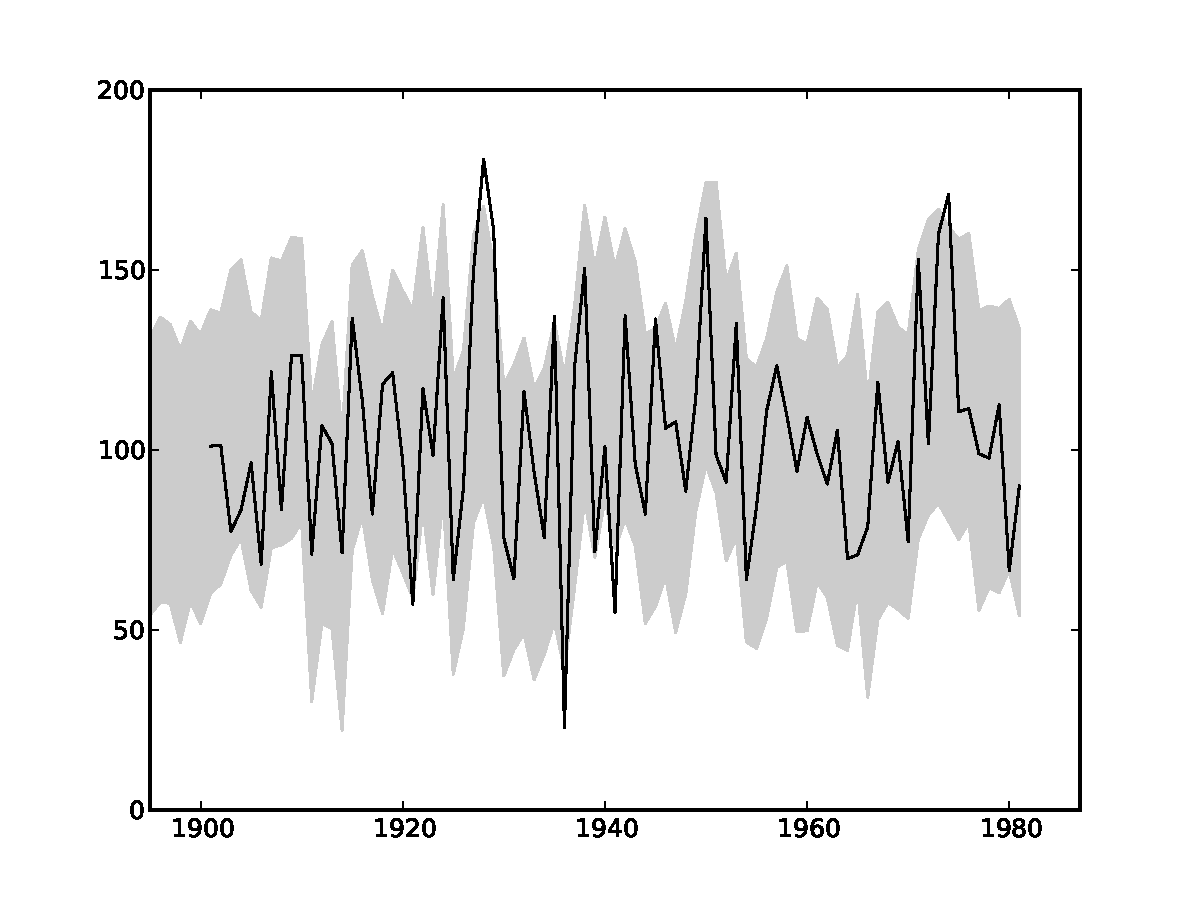
\includegraphics[width=6in]{figures/reconPrecip.pdf}
\caption{Average May-June precipitation (mjPR) reconstruction (blue line) and 95\% credible interval (grey lines). Precipitation data is plotted in red for years available (1901-1981).}
\label{fig:precipRecon}
\end{figure}

\begin{figure}
\centering
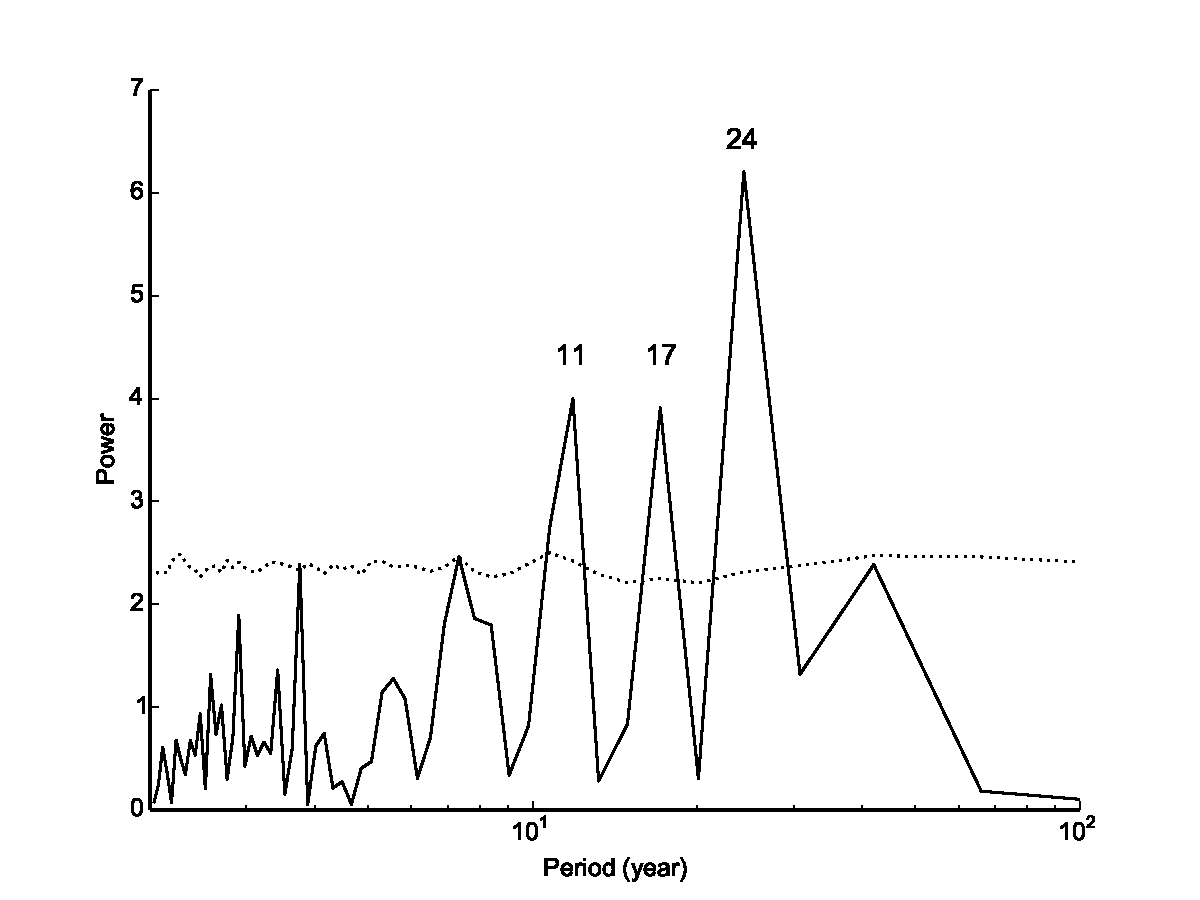
\includegraphics[width=6in]{figures/spectralRecon.pdf}
\caption{Periodogram showing periodicity of high amplitude at 46.2 and 23.1 years, as well as periodicity that is less pronounced with periods of 3.7, 7.5, 10.5, 11.6, and 12.2 years.}
\label{fig:spectral}
\end{figure}


\begin{figure}
\centering
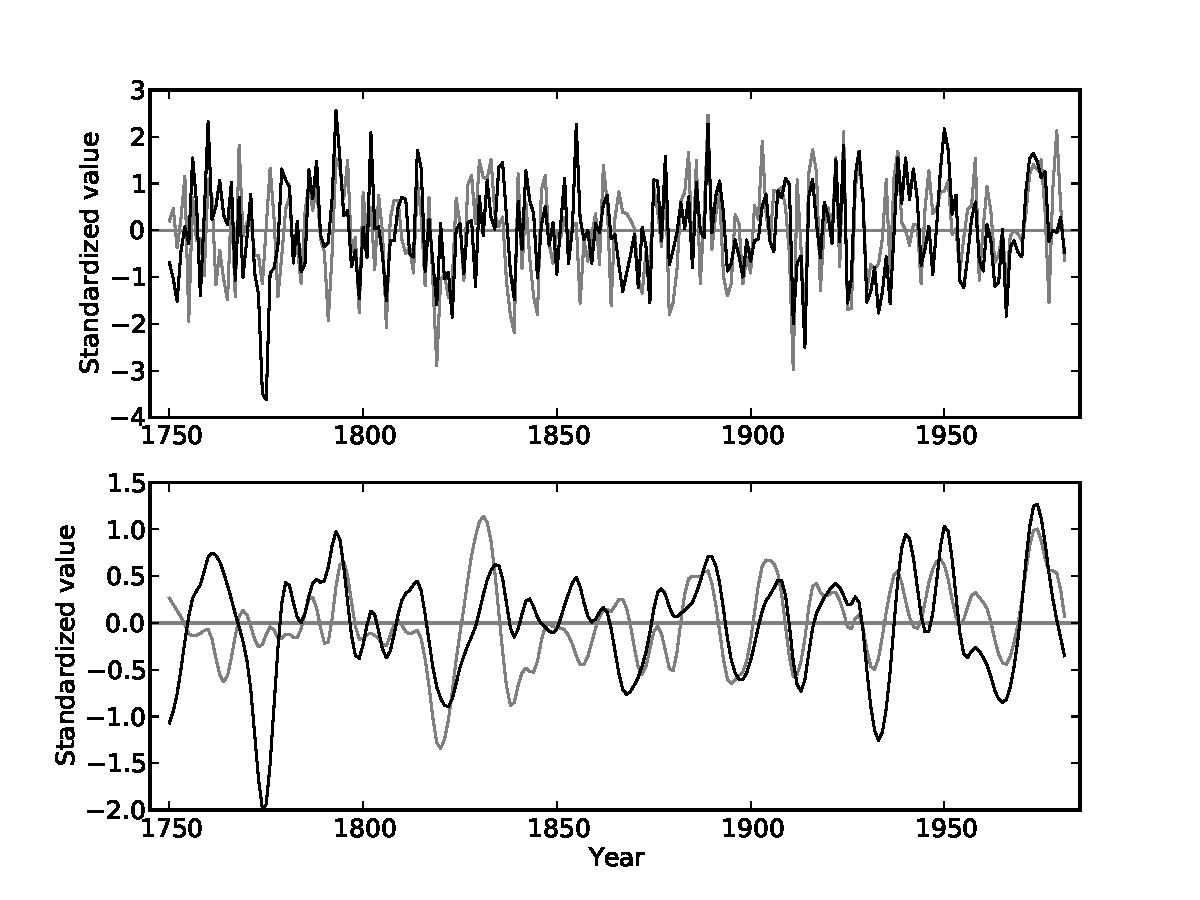
\includegraphics[width=6in]{figures/reconCompare.pdf}
\caption{Both the mjPR reconstruction and the Cook PDSI reconstruction are standardized and plotted against time to highlight both the similarities and the differences. Particularly notable differences include the year 1774, and the interval 1855-1863.}
\label{fig:reconCompare}
\end{figure}

\begin{figure}
\centering
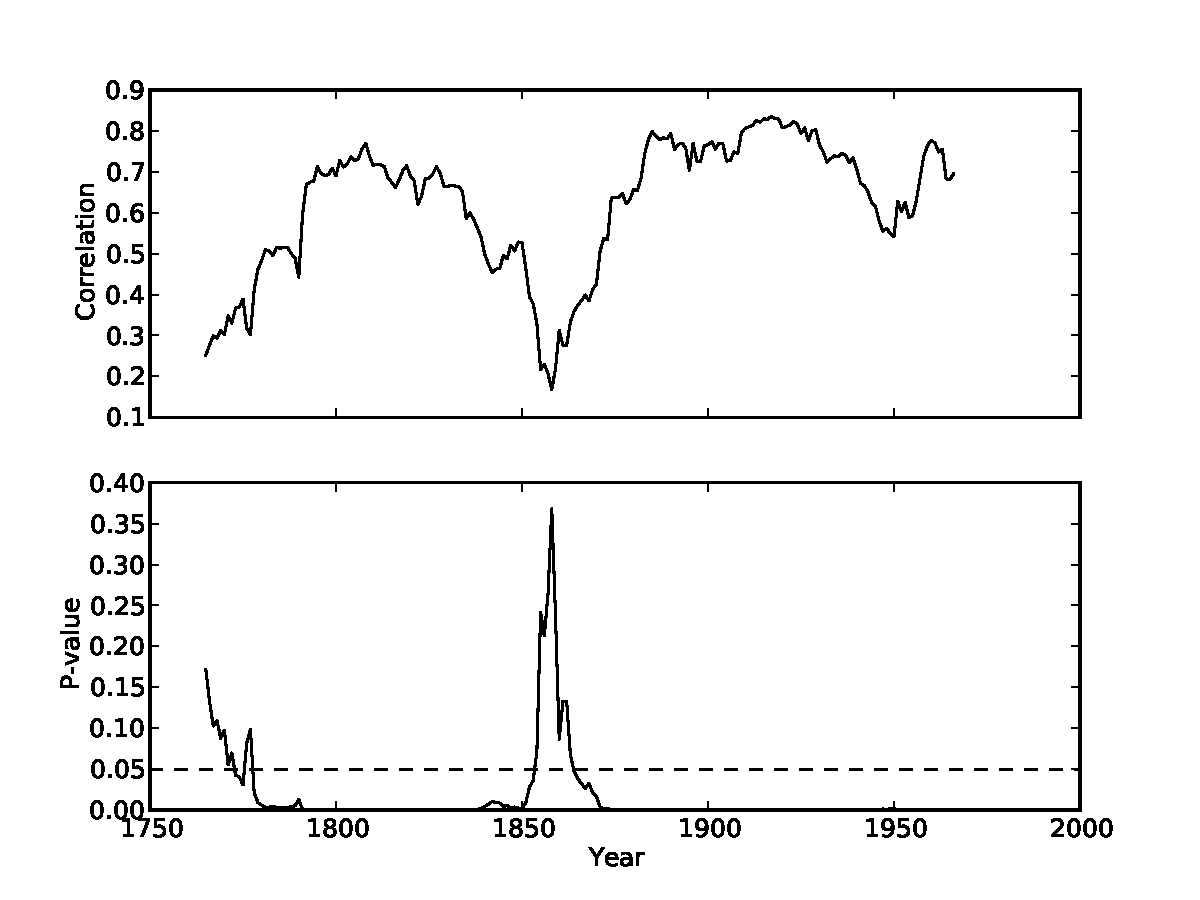
\includegraphics[width=6in]{figures/reconRunningCorr.pdf}
\caption{A 31 year windowed correlation plot between the mjPR and Cook PDSI reconstructions shows the discrepancy during the 1855-1863 interval. In the top panel correlation values are plotted about window centers, while the bottom panel shows the corresponding p-value (black) as well as the line of significance (red).}
\label{fig:reconRunningCorr}
\end{figure}

\begin{figure}
\centering
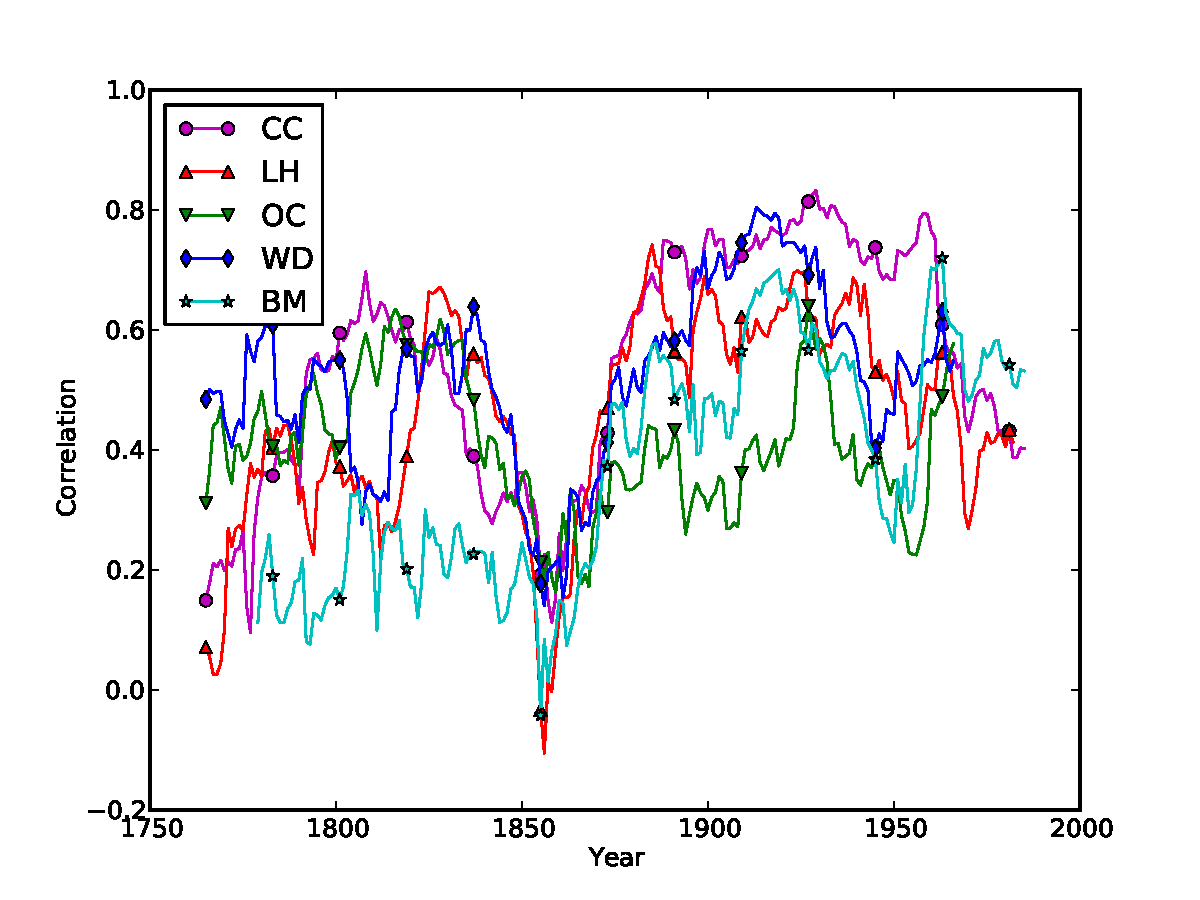
\includegraphics[width=6in]{figures/cookPdsiRunningCorr.pdf}
\caption{A 31 year windowed correlation plot between each of the chronologies and the Cook PDSI reconstruction. Note the interval of abrupt correlation during the years 1855-1863.}
\label{fig:cookRunningPdsiCorr}
\end{figure}

